%%%%%%%%%%%%%%%%%%%%%%%%%%%%%%%%%%%%%%%%%
% Beamer Presentation
% LaTeX Template
% Version 1.0 (10/11/12)
%
% This template has been downloaded from:
% http://www.LaTeXTemplates.com
%
% License:
% CC BY-NC-SA 3.0 (http://creativecommons.org/licenses/by-nc-sa/3.0/)
%
%%%%%%%%%%%%%%%%%%%%%%%%%%%%%%%%%%%%%%%%%

%----------------------------------------------------------------------------------------
%	PACKAGES AND THEMES
%----------------------------------------------------------------------------------------

\documentclass{beamer}

\mode<presentation> 
{

\usetheme{Madrid}

}
\usepackage{graphicx} % we need this so we can add figures
\usepackage{booktabs} % Allows the use of \toprule, \midrule and \bottomrule in tables
\usepackage{natbib} % we need this so we can use citation and bib properly
\usepackage{hyperref} % allows you to add hyperlink
\usepackage{amsmath} % allows you to use most mathematical features
\usepackage{setspace} % allows you to change the line spacing
\usepackage{longtable}
\usepackage{xr}
\usepackage{booktabs} % Allows the use of \toprule, \midrule and \bottomrule in tables
\usepackage{longtable}
\usepackage{threeparttable}
\usepackage{ragged2e}
\usepackage{caption}
\usepackage{subcaption} % for subfigures


\title[Kolloquium]{Conflict-Driven Evolution and Urban Development} % The short title appears at the bottom of every slide, the full title is only on the title page
\subtitle{Evidence from the Holy Roman Empire}

\author{Elias Hadj Ammar} % Your name

\institute[LMU] % Your institution as it will appear on the bottom of every slide, may be shorthand to save space
{
LMU Munich\\ % Your institution for the title page
\medskip
\textit{Elias.Ammar@campus.lmu.de} % Your email address
}
\date{August 3, 2023} % Date, can be changed to a custom date



\begin{document}

\begin{frame}
\titlepage % Print the title page as the first slide
\end{frame}

% no table of contents



%----------------------------------------------------------------------------------------
%	PRESENTATION SLIDES
%----------------------------------------------------------------------------------------


%------------------------------------------------
\section{Motivation} % 
%------------------------------------------------

\begin{frame}
\frametitle{Motivation}

\begin{itemize}
    \item Great Divergence: Europe vs. China and the rest
    \item One difference: balance of power, competition between states
\end{itemize}

\end{frame}

% the motivation needs to be clear even when the audience doesn't know yet what the question is!

\begin{frame}
\frametitle{Motivation}

\begin{figure}
     \centering
     \begin{subfigure}[b]{0.3\textwidth}
         \centering
         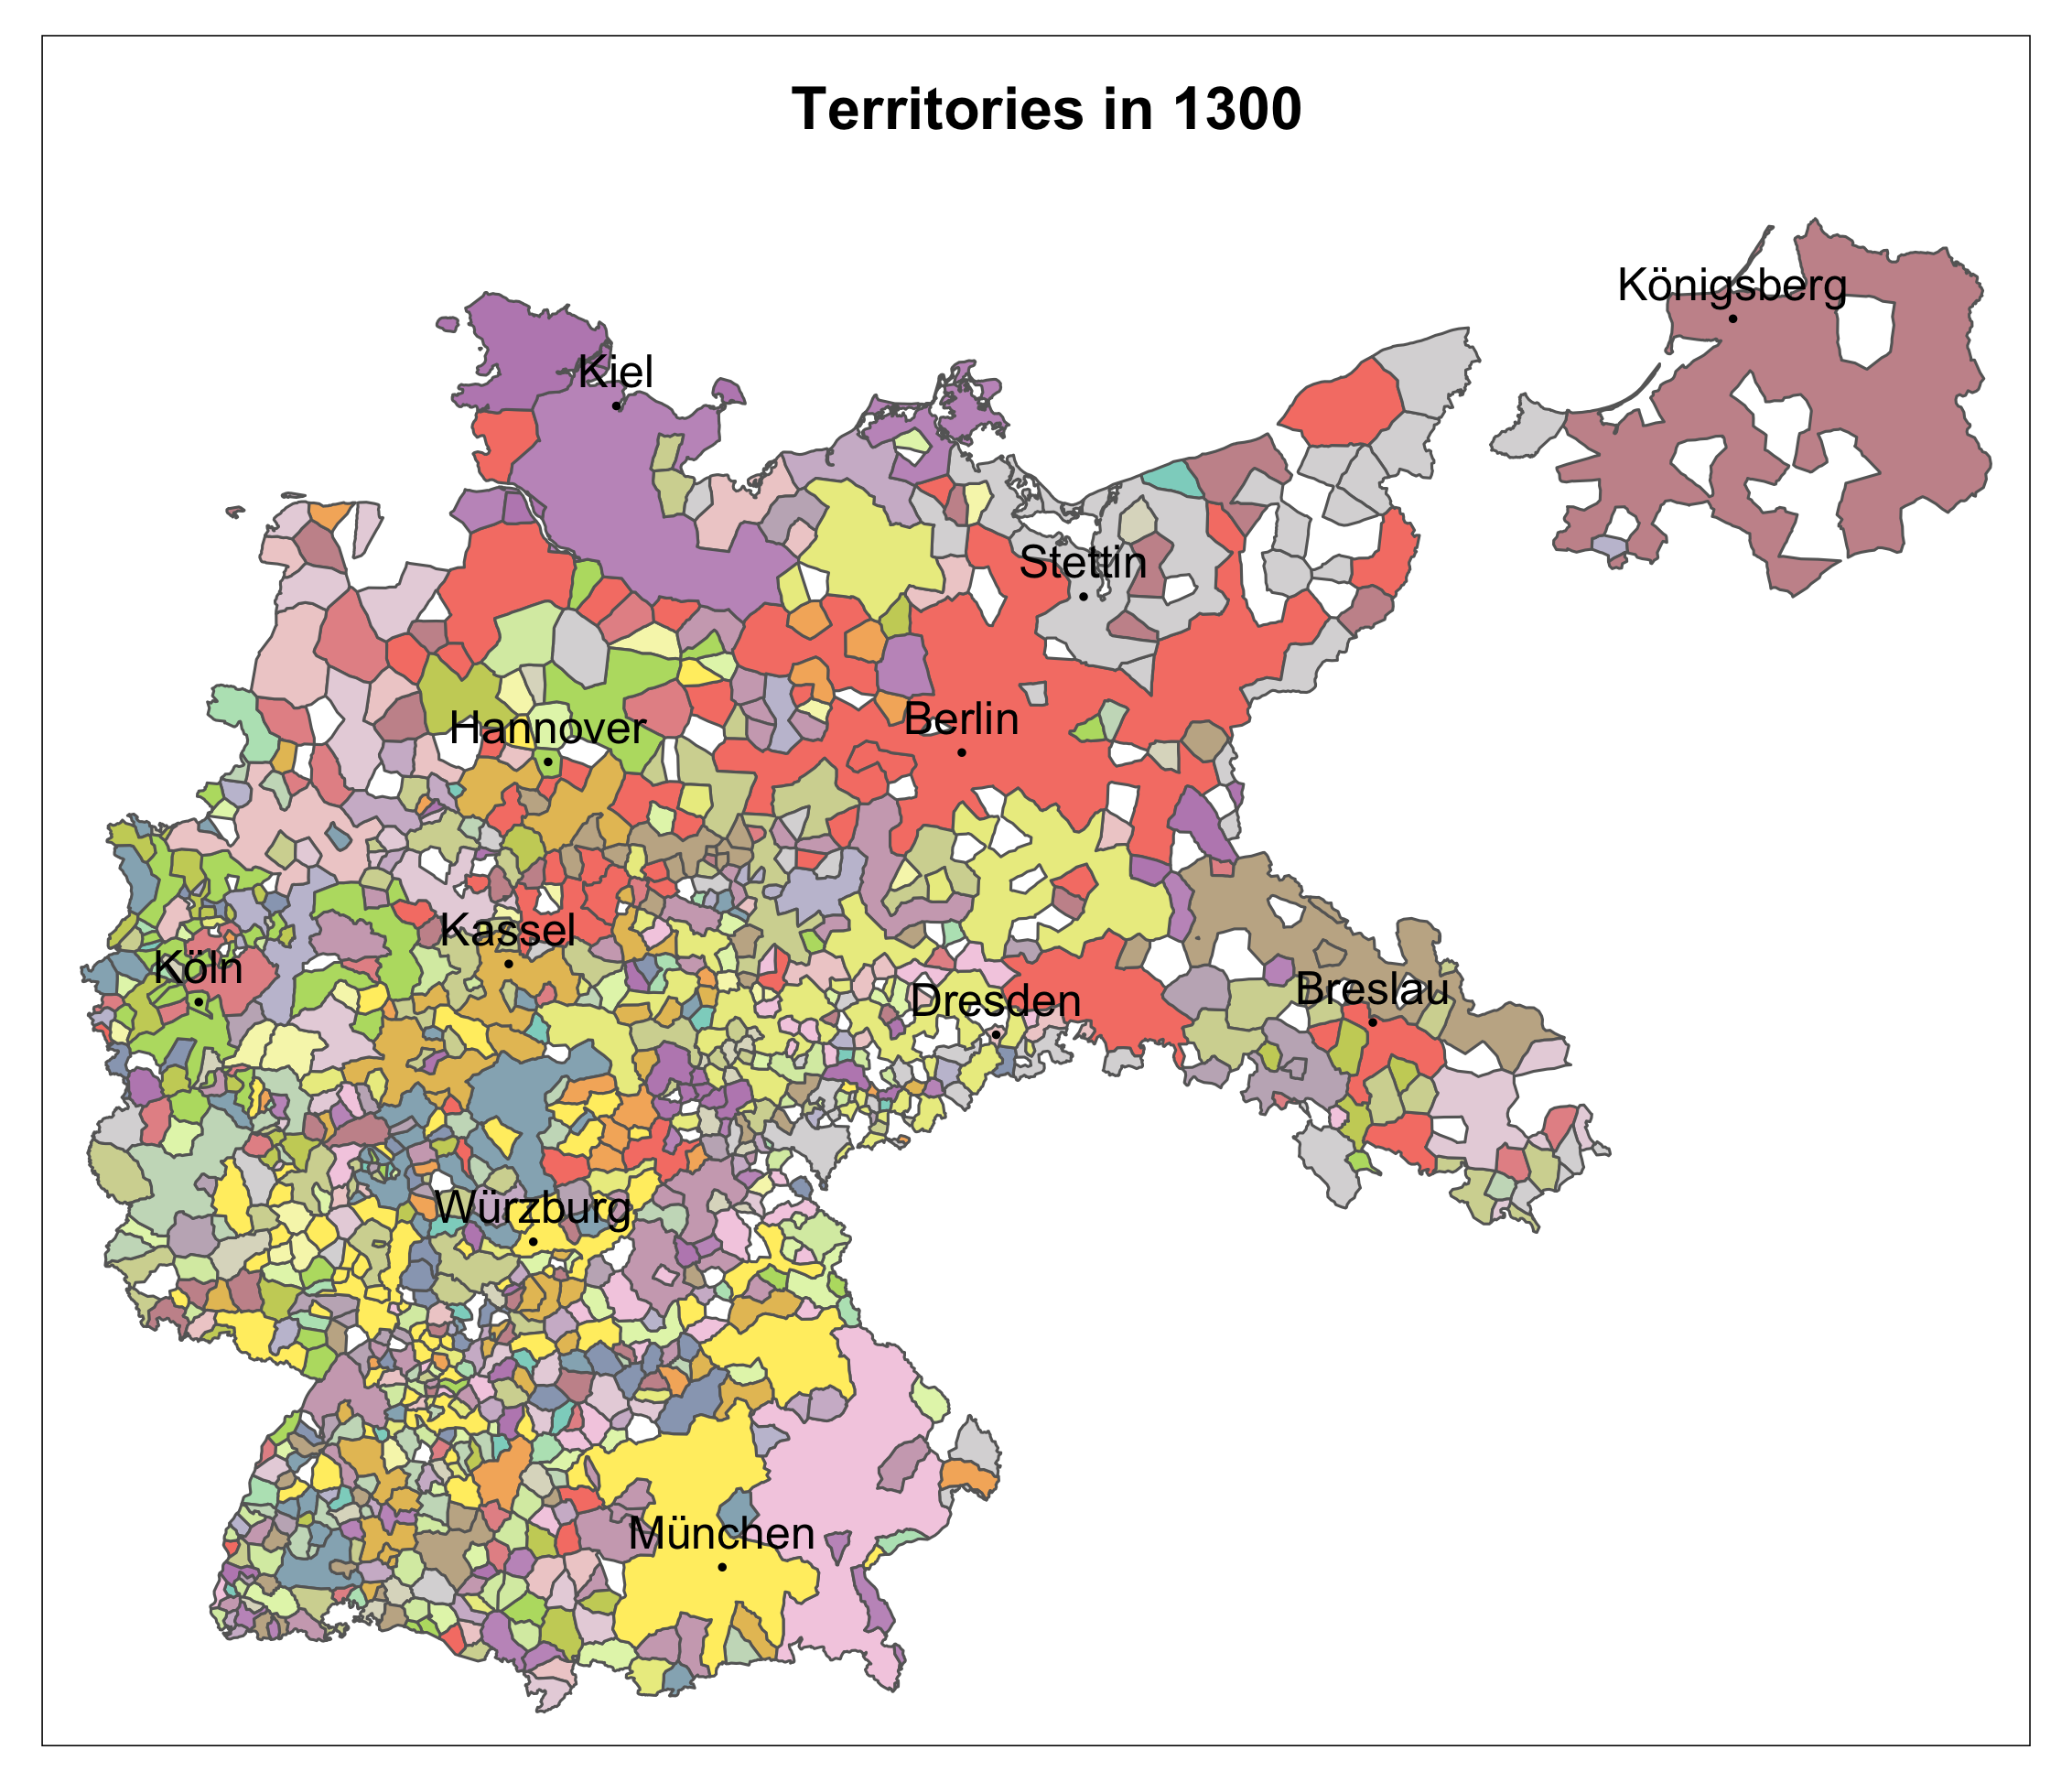
\includegraphics[width=\textwidth]{paper/output/slides/map_terrs_1300.png}
         \caption{1300}
         \label{fig:map1300}
     \end{subfigure}
     \hfill
     \begin{subfigure}[b]{0.3\textwidth}
         \centering
         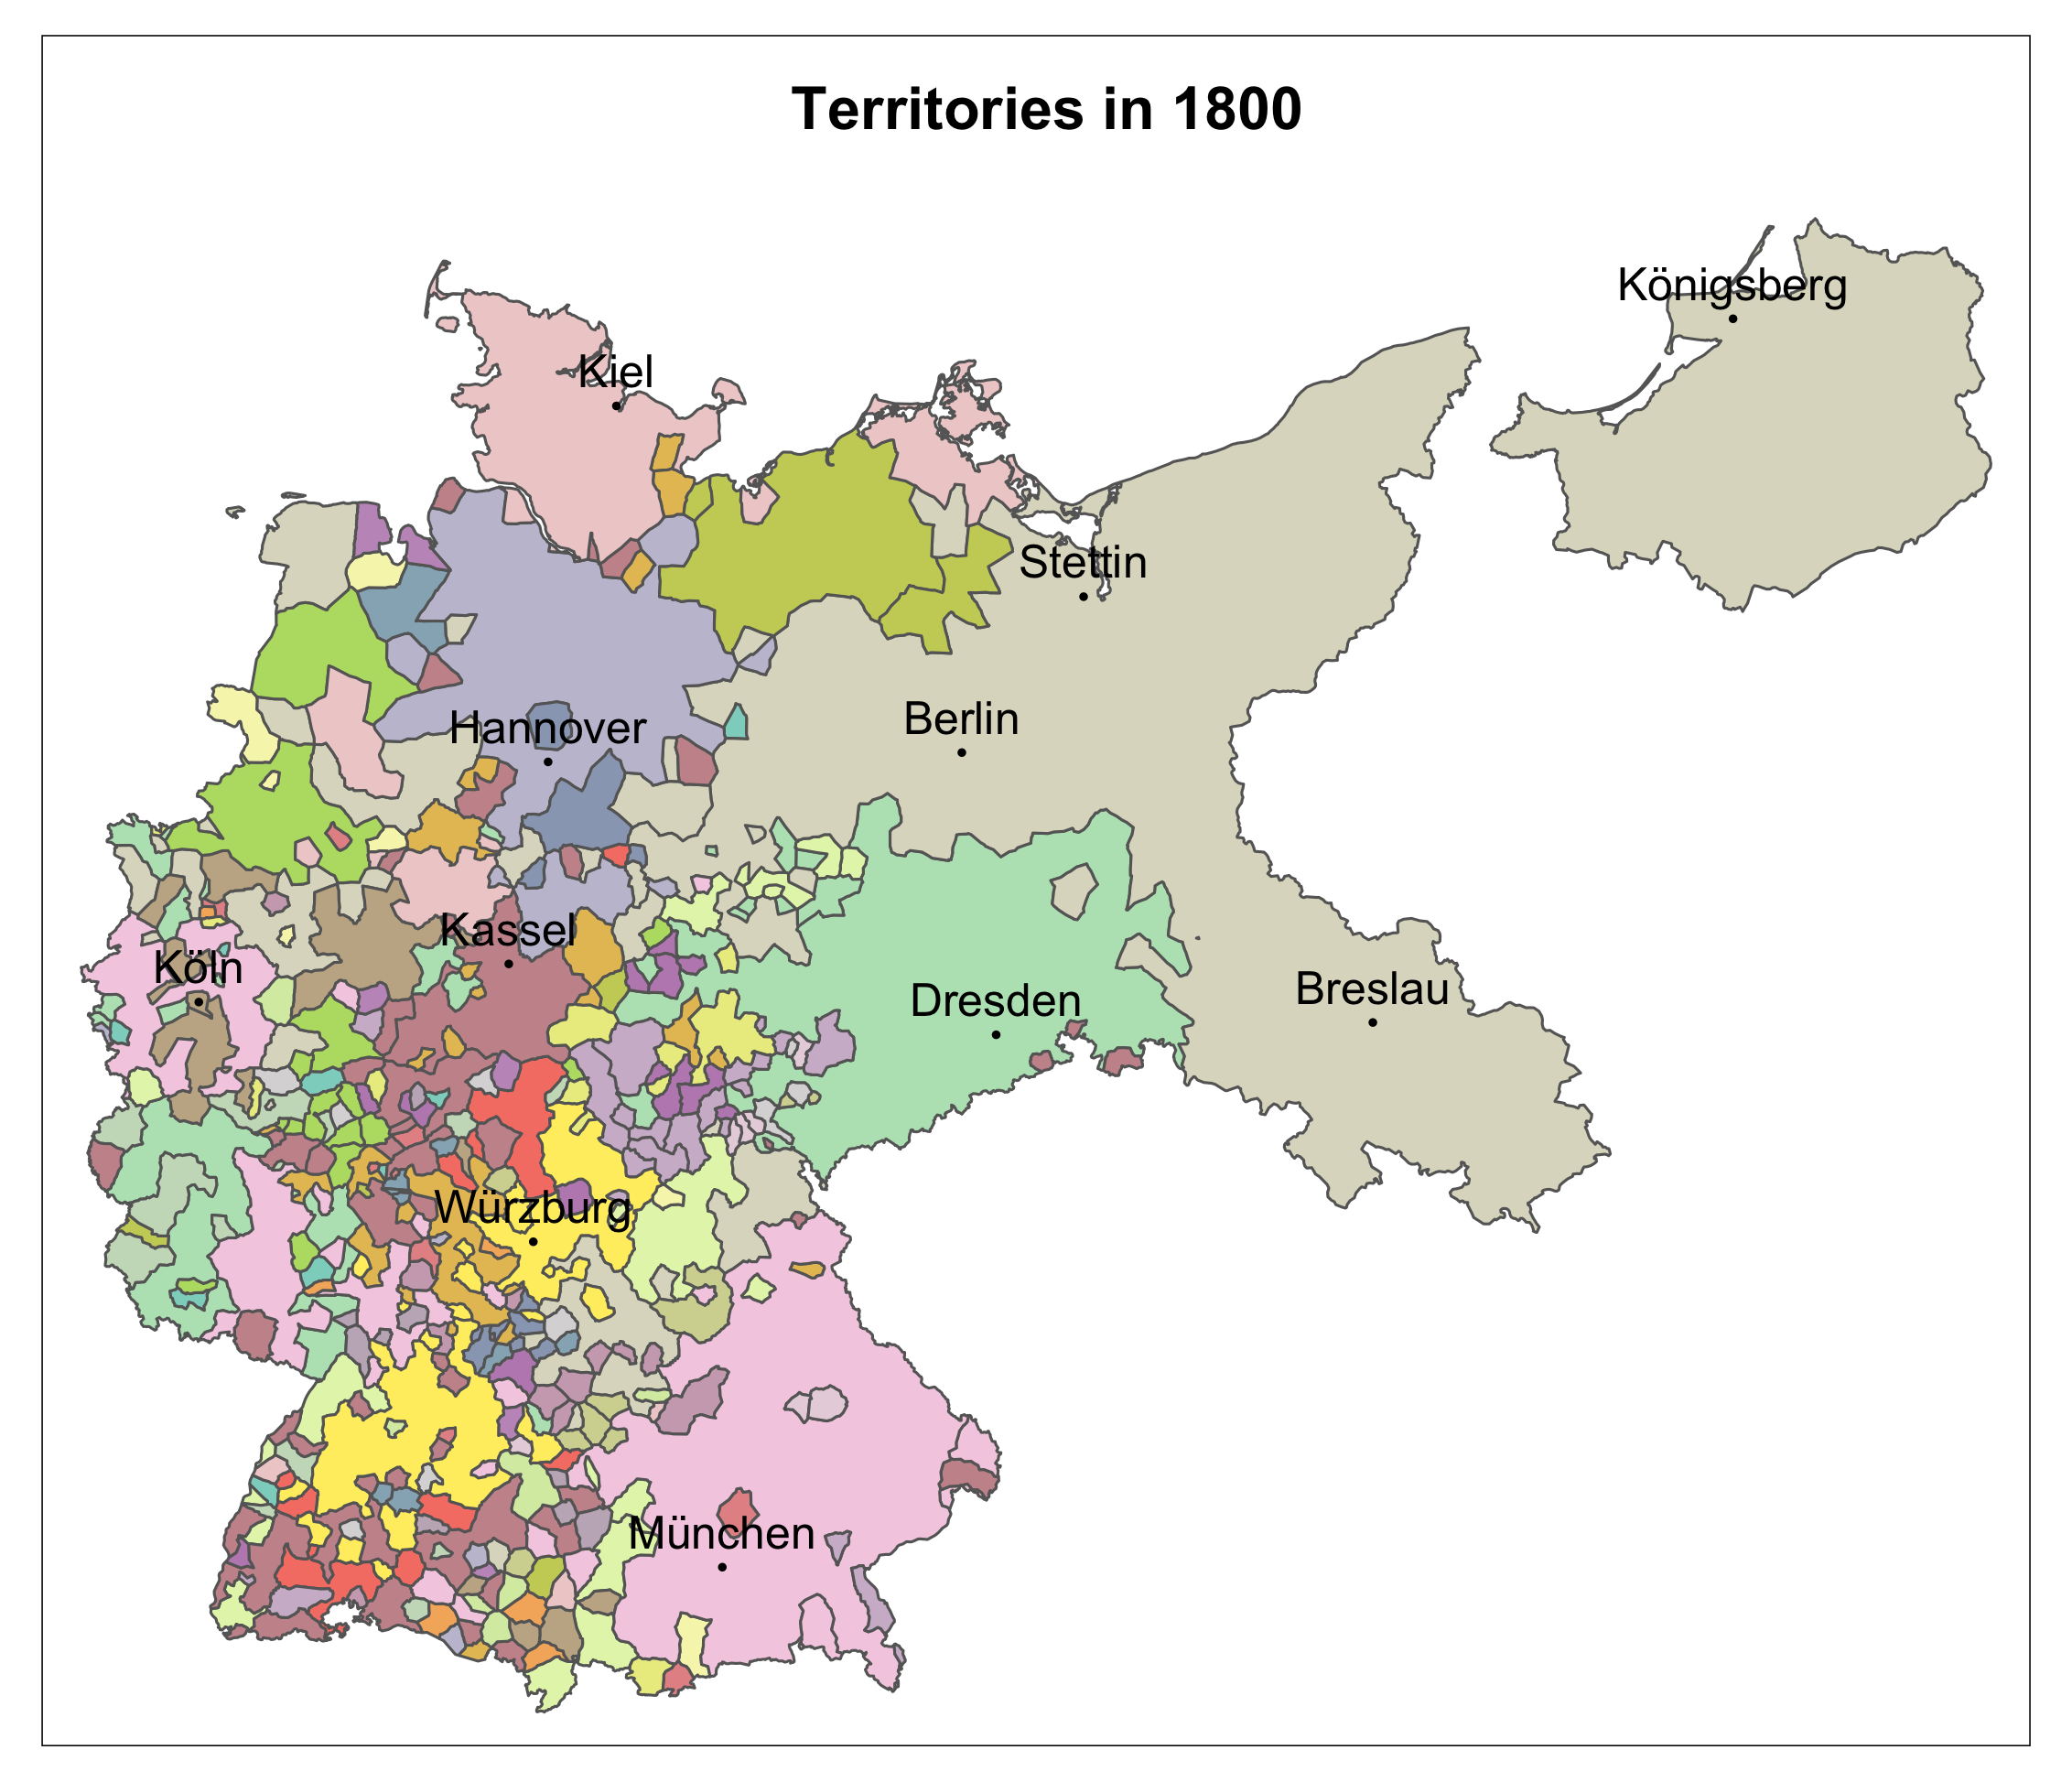
\includegraphics[width=\textwidth]{paper/output/slides/map_terrs_1800.png}
         \caption{1800}
         \label{fig:map1800}
     \end{subfigure}
    \hfill
     \begin{subfigure}[b]{0.3\textwidth}
         \centering
         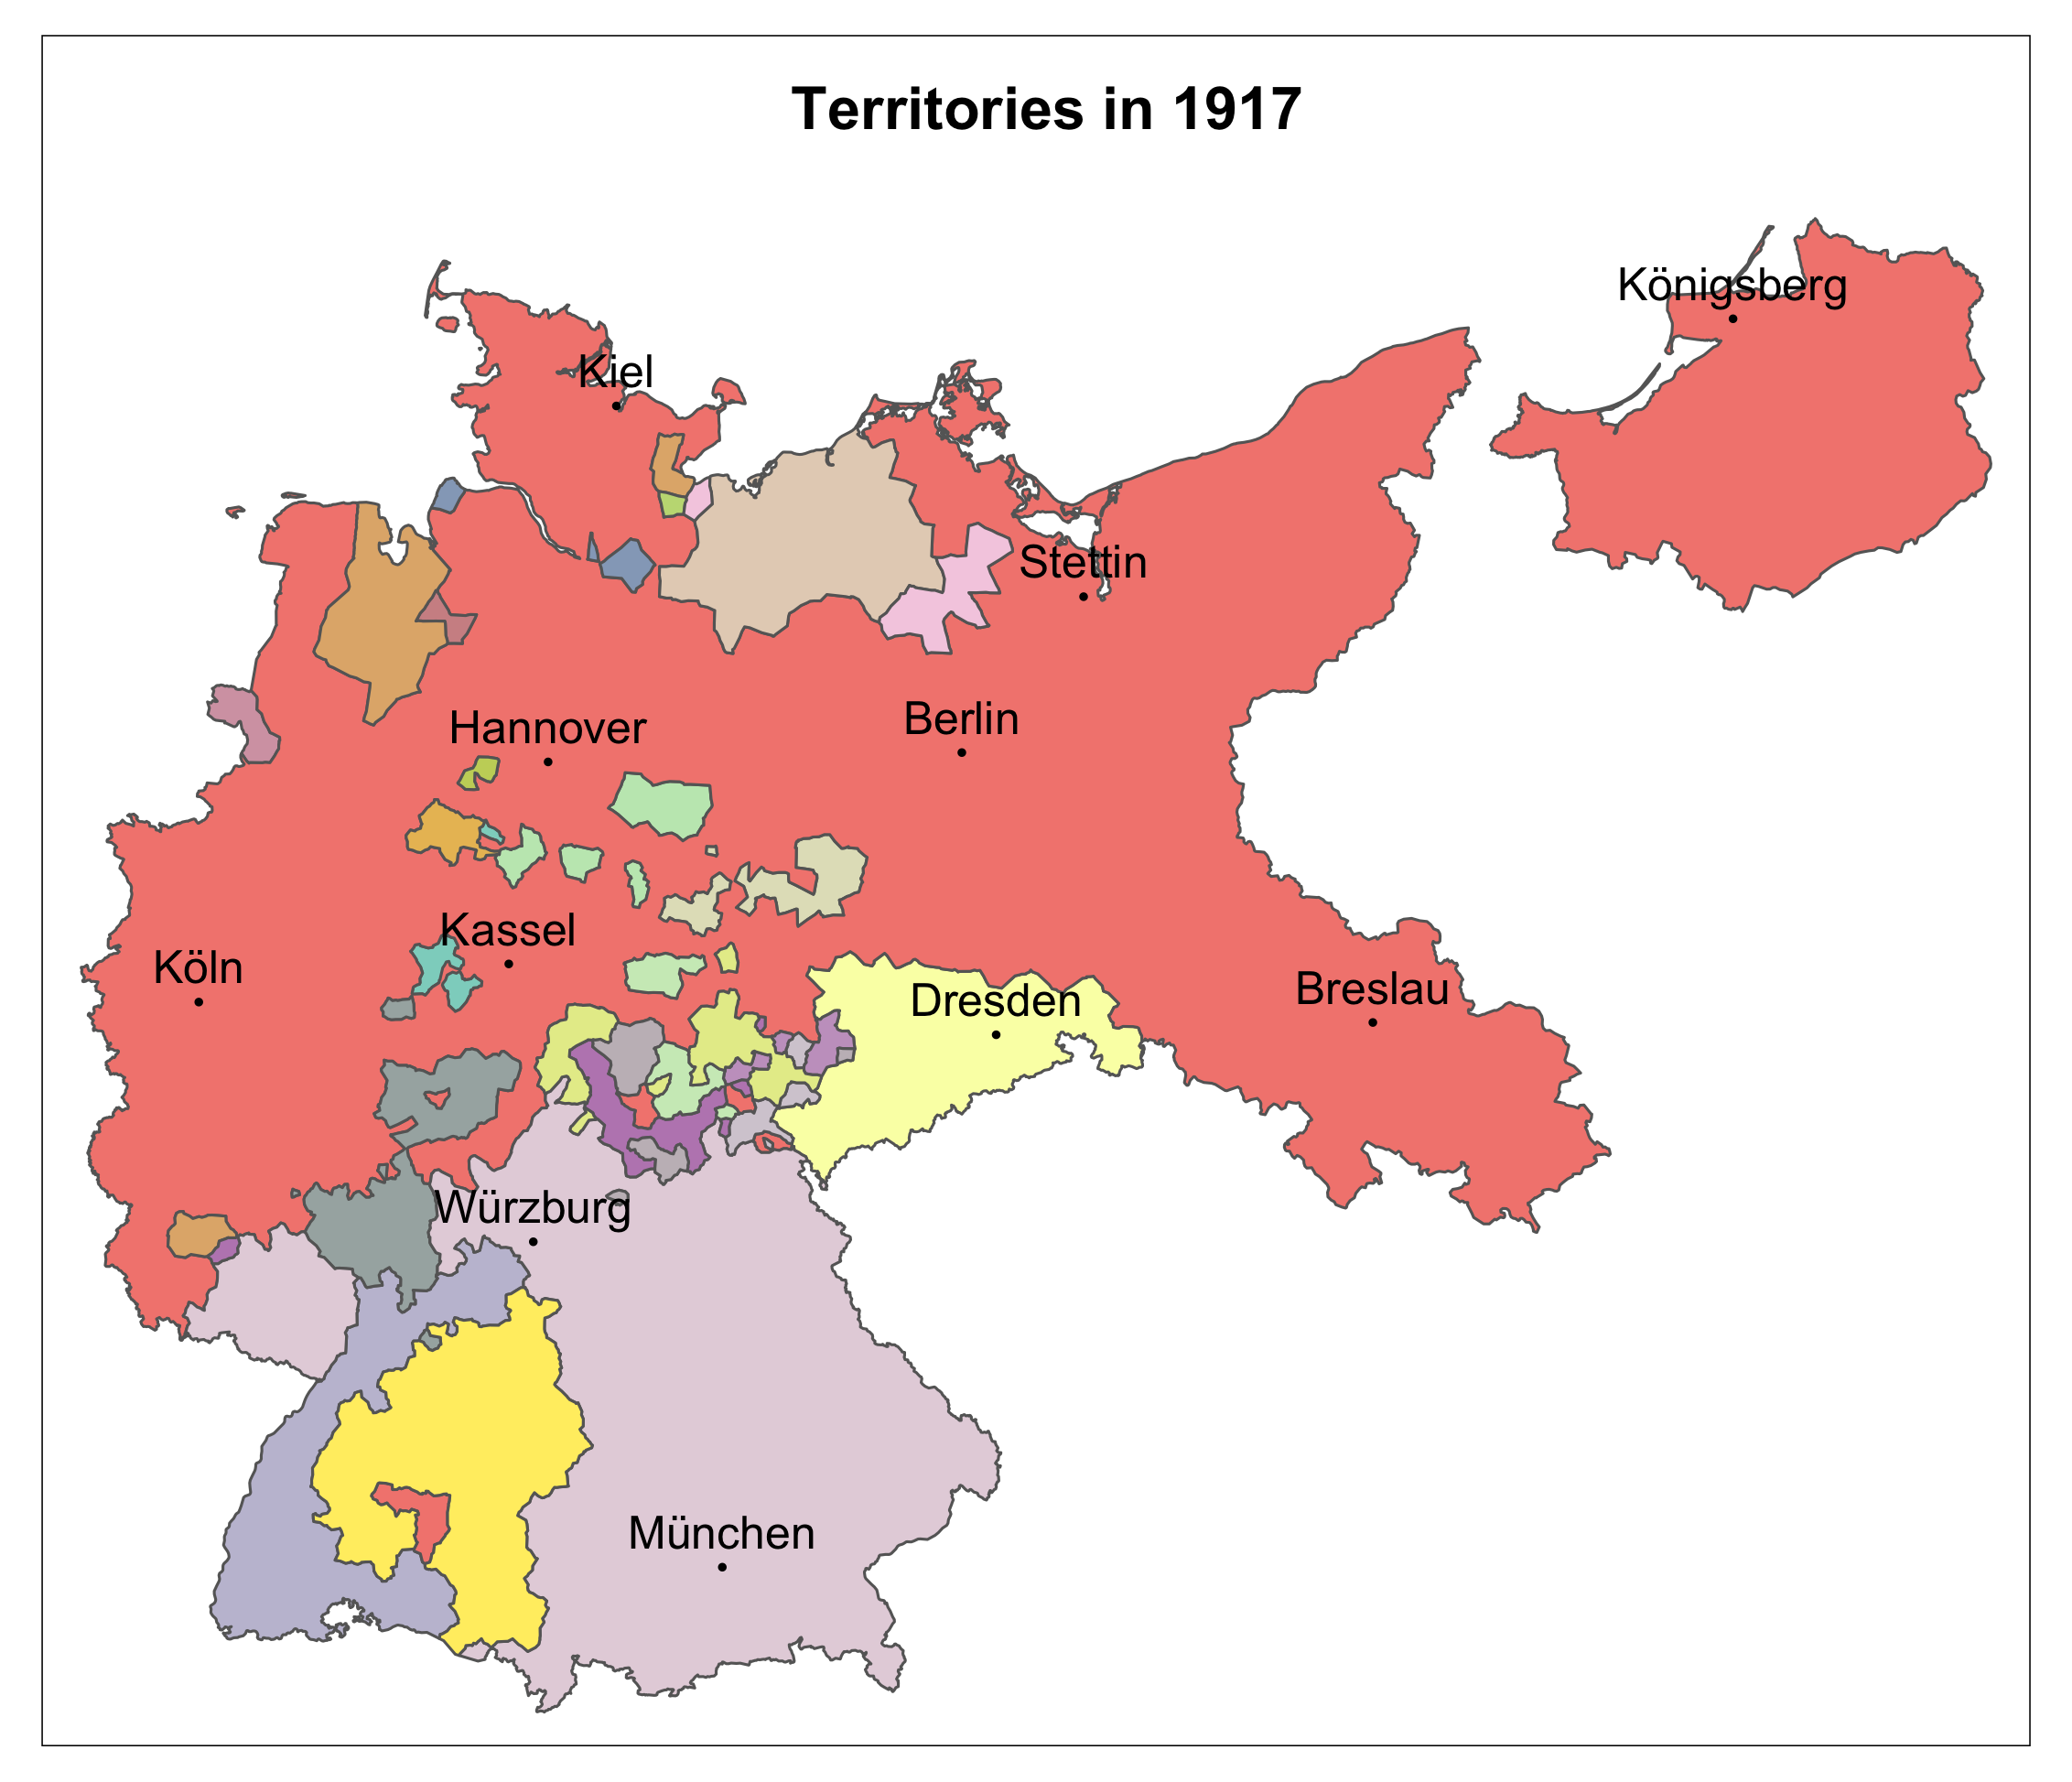
\includegraphics[width=\textwidth]{paper/output/slides/map_terrs_1917.png}
         \caption{1917}
         \label{fig:map1917}
     \end{subfigure}
        \caption{Territorial history of the German Empire}
        \label{fig:terrmaps}
\end{figure}
    
\end{frame}

\begin{frame}
\frametitle{Motivation}



\begin{itemize}
    \item states struggle for resources (=territory)
    \item some states survive and grow, others get eaten
   \item survival of the fittest: selection for strength / power\footnote[frame,1]{\cite{levine2021}}
\end{itemize}
    
\end{frame}


%------------------------------------------------
\section{Outline} % 
%------------------------------------------------

\begin{frame}
\frametitle{This paper}
\justifying
$\rightarrow$ \textbf{Question}: 
Did this process play a role in the rise of Europe?
\medskip
\begin{itemize}
\item Wars = weak states getting eaten by better ones
\item Maybe "stronger" states are richer (institutions?) 
\item Darwinian selection caused state quality in Europe to constantly improve
\end{itemize}

\end{frame}

%------------------------------------------------


\begin{frame}
\frametitle{Positive View: }

\begin{block}{Point 3}
Here briefly mention one main positive view
\end{block}

if you want to add graphs, it is the same procedure as when you write your essay. Make sure you adjust the size so your classmates can see it properly.
\begin{figure}[hbt!]
    \centering
    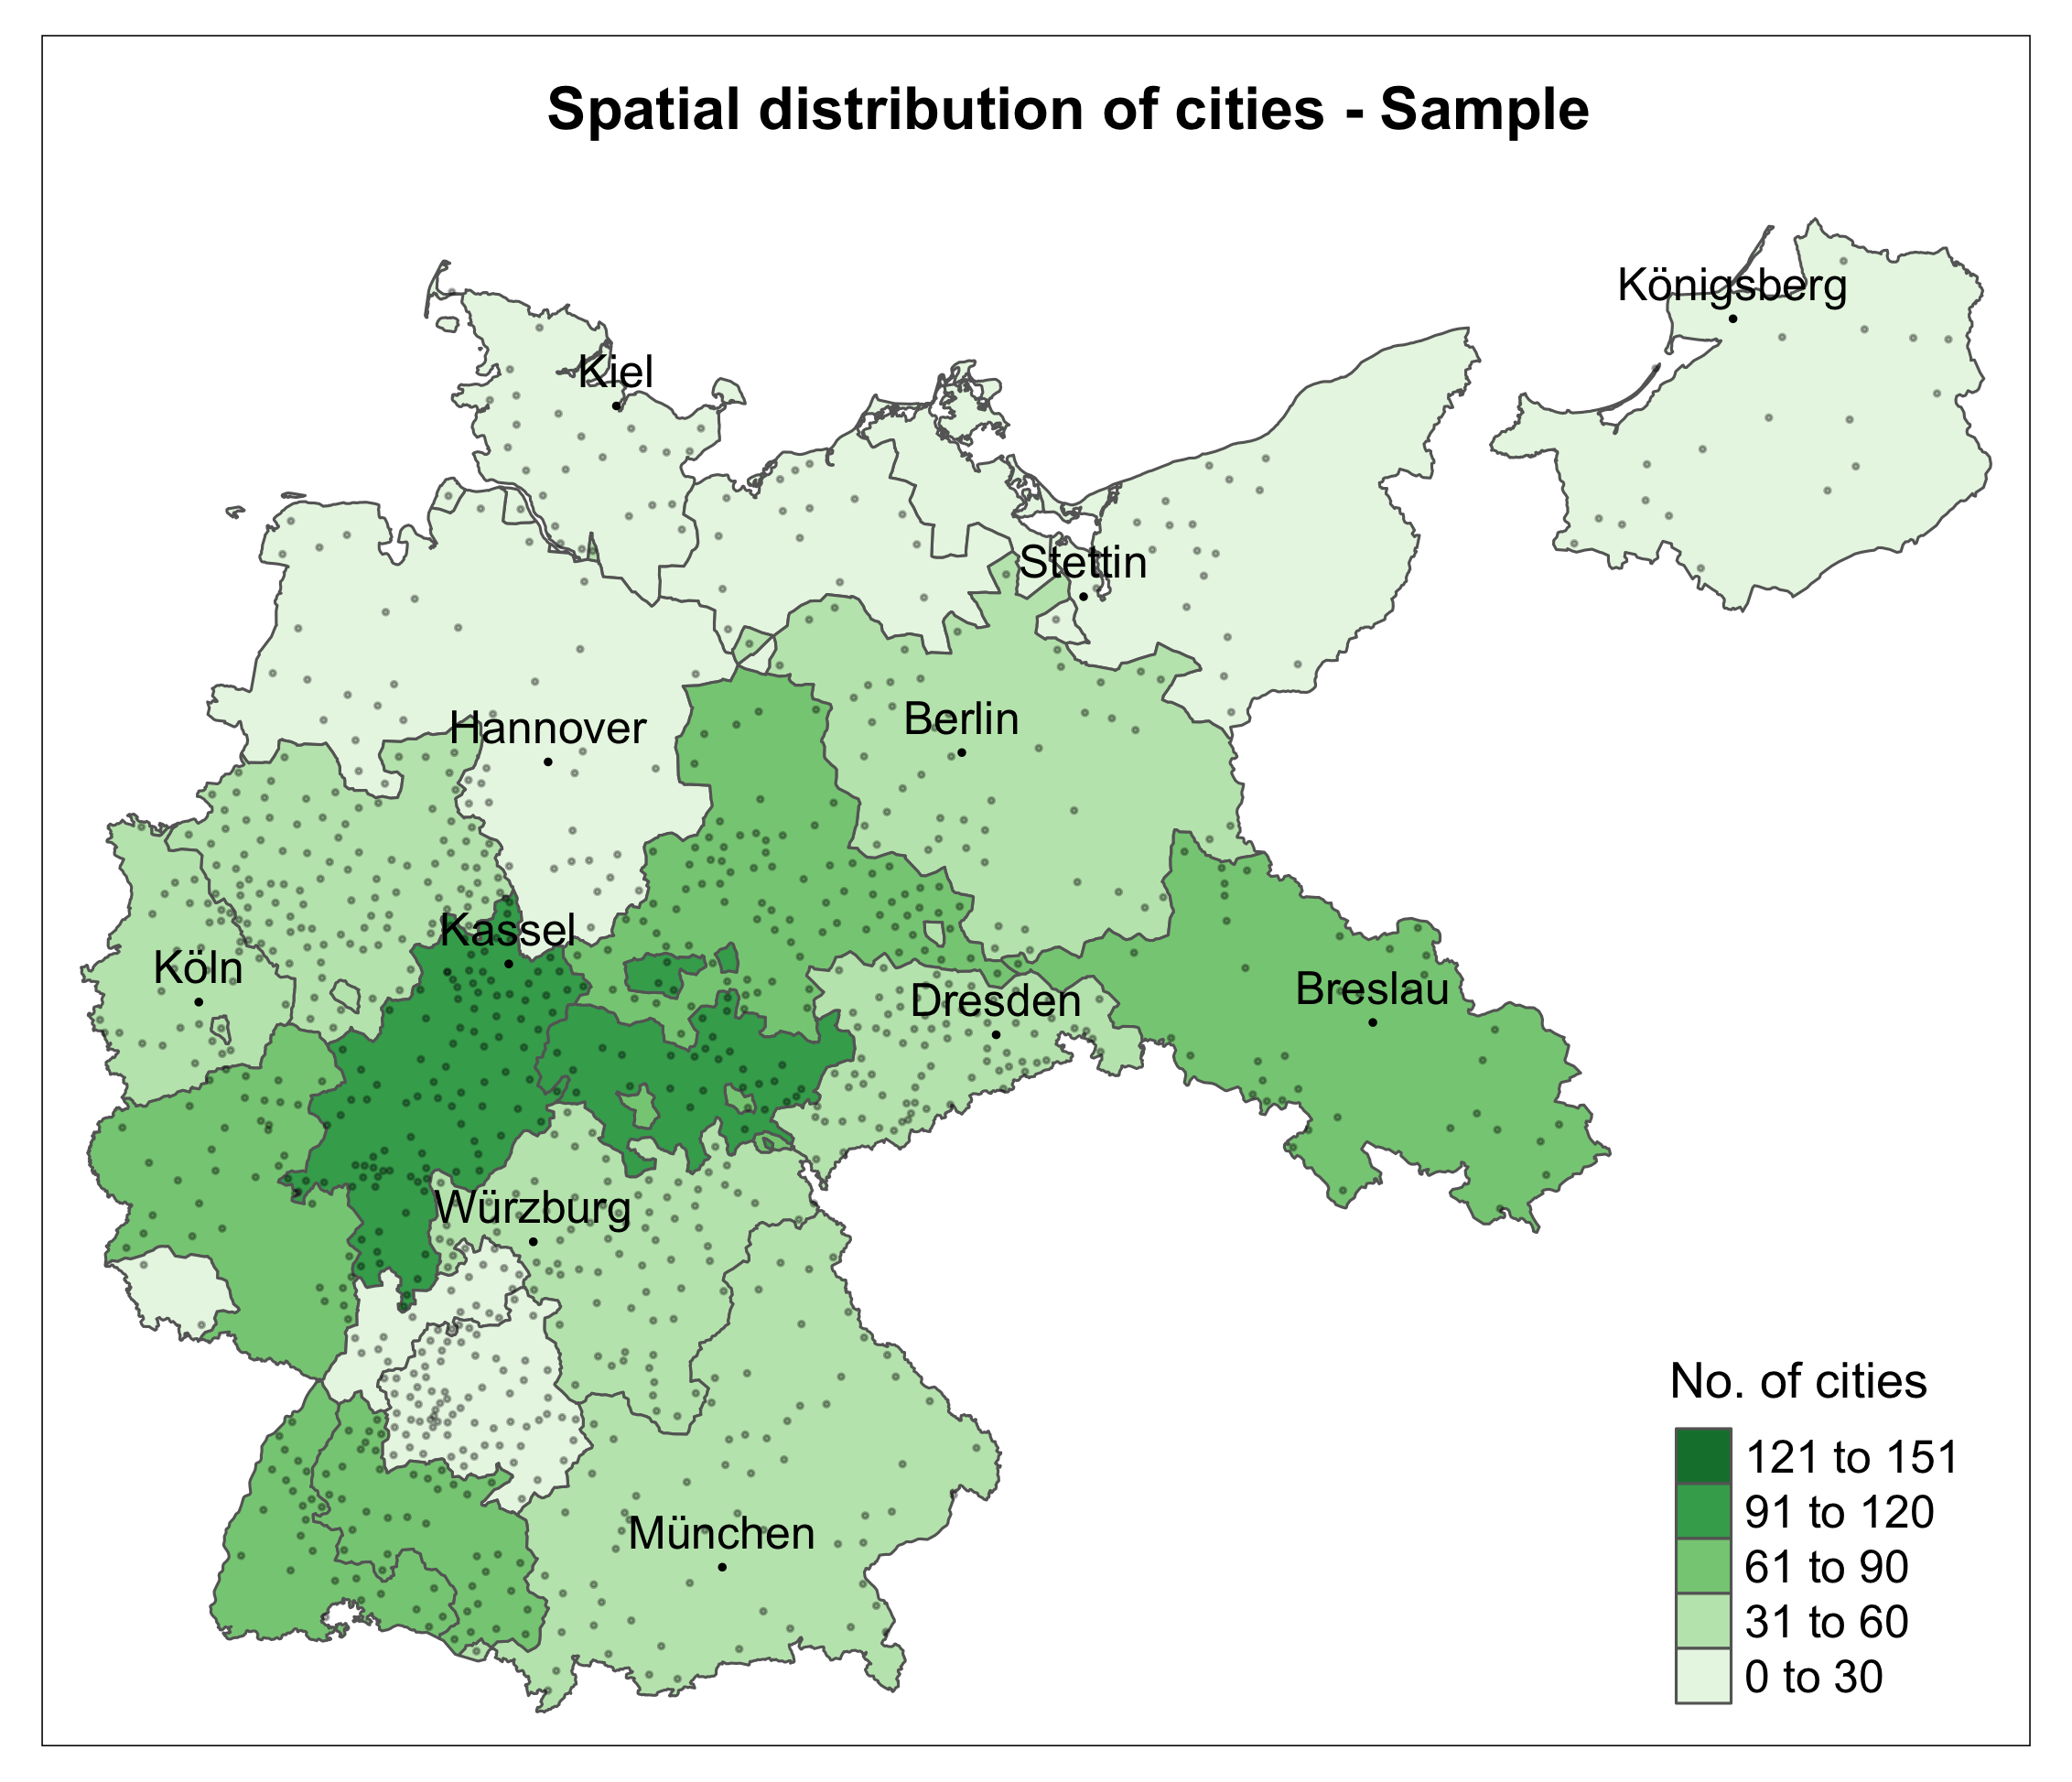
\includegraphics[width=0.3\textwidth]{paper/output/descriptive/map_cities_sample.png}
    \caption{The composition of migrants and the provision of common schools; Source: me}.
    \label{table:my_label}
\end{figure}

\end{frame}

%------------------------------------------------

\begin{frame}
\frametitle{Positive View: }
You can also draw a table yourself

\begin{table}
\begin{tabular}{l l l}
\toprule
\textbf{Treatments} & \textbf{Response 1} & \textbf{Response 2}\\
\midrule
Treatment 1 & 0.0003262 & 0.562 \\
Treatment 2 & 0.0015681 & 0.910 \\
Treatment 3 & 0.0009271 & 0.296 \\
\bottomrule
\end{tabular}
\caption{Table caption}
\end{table}

\end{frame}



%------------------------------------------------
\section{End}% 
%------------------------------------------------

\begin{frame}
\frametitle{References}
\justifying

\bibliography{paper/references}
\bibliographystyle{chicago}

\end{frame}

%------------------------------------------------

\begin{frame}
\Huge{\centerline{The End}}
\end{frame}

%----------------------------------------------------------------------------------------

%------------------------------------------------
\section{Appendix}% 
%------------------------------------------------



\end{document}